
\label{Sec:introDataScience}
%\subsection{Brief Introduction to Data Science}
\lehrtext{Data science as a field has far more applications than quality management, however quality management professionals take huge advantages from the application of data science tools and methods in their daily and non-daily work.

For this reason, enjoy this brief introduction and the more thorough hands-on training provided in the sequel!
}

\frame{\frametitle{What is Data Science?}
\lehrtext{Data science is our means of taming unstructured information and gathering insight. - Matthew Mayo, KDnuggets}
\begin{itemize}
\item Interdisciplinary field of
\begin{itemize}
		\item Systems,
		\item Methods and
		\item Processs to extract insight or knowledge from data.
\end{itemize}
\item Term coined in 2001, gained popularity in 2010
\item Integrates:
\begin{itemize}
		\item Data Engineering
		\item Scientific Method
		\item Mathematics
		\item Statistics
		\item Advanced Computational Methods
		\item Visualisation
		\item Hacker Mindset
		\item Domain Expertise
		\end{itemize}
\end{itemize}
}


\frame{\frametitle{How does Data Science integrate to Mechanical Engineering?}
\lehrtext{You may ask yourself: what is the point in learning to code in Python and apply data science tools, I am a mechanical engineer?

The short answer is: you will probably need it.

The longer answer is: your domain expertise, coupled with the willingness to dive into data, makes the difference!}

\begin{center}
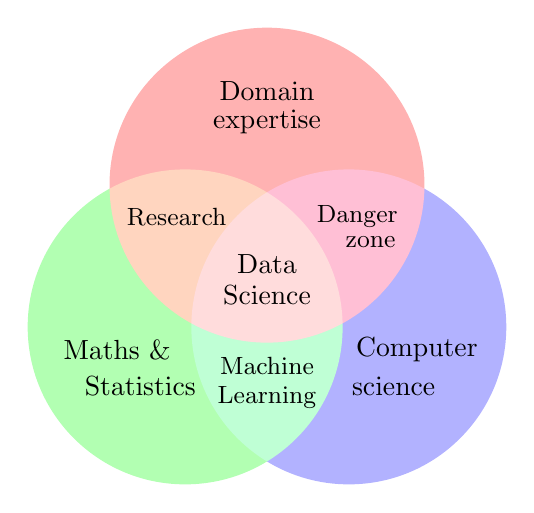
\begin{tikzpicture}
\begin{scope}[blend group=soft light]
\fill[red!30!white] ( 90:1.2) circle (2); 
\fill[green!30!white] (210:1.2) circle (2); 
\fill[blue!30!white] (330:1.2) circle (2); 
\end{scope}
%\node at ( 90:2.6) {Railway}; 
\node at ( 90:2.4) {Domain}; 
\node at ( 90:2.0) {expertise}; 
\node at (205:2.1) {Maths \&};
\node at (220:2.1) {Statistics}; 
\node at (335:2.1) {Computer}; 
\node at (320:2.1) {science}; 
%\node at (0,.4) {Rail};
\node at (0,0.2) {Data};
\node at (0,-.2) {Science};
\node at (270:1.1) {\small Machine};
\node at (270:1.5) {\small Learning};
\node at (145:1.4) {\small Research};
\node at (35:1.4) {\small Danger};
\node at (20:1.4) {\small zone};
\end{tikzpicture}
\end{center}
}

\frame{\frametitle{Why Data Sciene?}
\lehrtext{In a company context, you frequently act without proper information, although it is there - just nobody takes the time to analyse it. As soon as you show up to a board meeting or similar with data, people tend to trust your claims and you may be the one who is heard.

As Deming (the guy with the PDCA circle...) said:

\begin{quotation}
\textbf{In God we trust, all others bring data.}
\end{quotation}

Data science puts you in a position to:
}
\begin{columns}[t] 
     \begin{column}[T]{6cm} 
     	\begin{itemize}
     		\item Turn data to information
		\begin{itemize}
		\item Inform decisions
		\item Increase insight
		\end{itemize}
		\item Companies:
		\begin{itemize}
		\item Collect large amounts of data
		\item Do rarely integrate them
		\item Frequently decide based on the ``gut''
		\end{itemize}
     	\end{itemize}
     \end{column}
     	\begin{column}[T]{6cm} 
	\only<beamer>{
         	\begin{center}
            		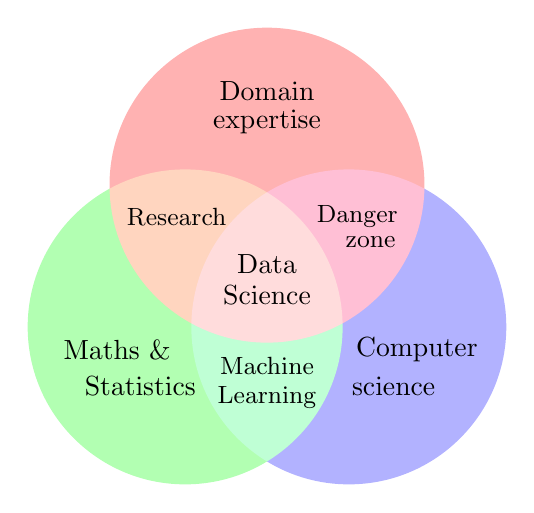
\begin{tikzpicture}
                            \begin{scope}[blend group=soft light]
                            \fill[red!30!white] ( 90:1.2) circle (2); 
                            \fill[green!30!white] (210:1.2) circle (2); 
                            \fill[blue!30!white] (330:1.2) circle (2); 
                            \end{scope}
                            %\node at ( 90:2.6) {Railway}; 
                            \node at ( 90:2.4) {Domain}; 
                            \node at ( 90:2.0) {expertise}; 
                            \node at (205:2.1) {Maths \&};
                            \node at (220:2.1) {Statistics}; 
                            \node at (335:2.1) {Computer}; 
                            \node at (320:2.1) {science}; 
                            %\node at (0,.4) {Rail};
                            \node at (0,0.2) {Data};
                            \node at (0,-.2) {Science};
                            \node at (270:1.1) {\small Machine};
                            \node at (270:1.5) {\small Learning};
                            \node at (145:1.4) {\small Research};
                            \node at (35:1.4) {\small Danger};
                            \node at (20:1.4) {\small zone};
                            \end{tikzpicture}

        		\end{center}}
     \end{column}
 \end{columns}
}

\frame{\frametitle{How do you increase Value with Data Science?}
\lehrtext{You are about to become engineers bearing the second highest education level in the EU (and world wide, for most countries) - perhaps you should bear in mind that the additional income and employer attractiveness come with some expectation: you are supposed to create value commensurate with your salary expectation and also your education level. Data Science may be helpful in this context.}
\begin{columns}[t] 
     \begin{column}[T]{6cm} 
     	\begin{itemize}
     		\item Improve decision making
		\begin{itemize}
		\item Empower management
		\item Supply data driven evidence
		\end{itemize}
		\item Identify trends and bring to action
		\item Challenge your colleagues
		\item Find opportunities for improvement
		\item Test decisions
		\item Understand customers
     	\end{itemize}
     \end{column}
     	\begin{column}[T]{6cm} 
	\only<beamer>{
         	\begin{center}
            		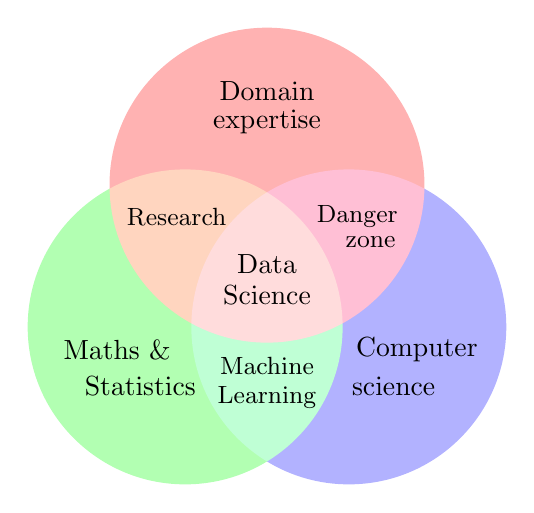
\begin{tikzpicture}
                            \begin{scope}[blend group=soft light]
                            \fill[red!30!white] ( 90:1.2) circle (2); 
                            \fill[green!30!white] (210:1.2) circle (2); 
                            \fill[blue!30!white] (330:1.2) circle (2); 
                            \end{scope}
                            %\node at ( 90:2.6) {Railway}; 
                            \node at ( 90:2.4) {Domain}; 
                            \node at ( 90:2.0) {expertise}; 
                            \node at (205:2.1) {Maths \&};
                            \node at (220:2.1) {Statistics}; 
                            \node at (335:2.1) {Computer}; 
                            \node at (320:2.1) {science}; 
                            %\node at (0,.4) {Rail};
                            \node at (0,0.2) {Data};
                            \node at (0,-.2) {Science};
                            \node at (270:1.1) {\small Machine};
                            \node at (270:1.5) {\small Learning};
                            \node at (145:1.4) {\small Research};
                            \node at (35:1.4) {\small Danger};
                            \node at (20:1.4) {\small zone};
                            \end{tikzpicture}

        		\end{center}}
     \end{column}
 \end{columns}
}

\frame{\frametitle{The data science process}
\lehrtext{The data science process starts with \emph{real world data}, which is messy, has missing values and all other ugly properties. So most of the time, you need to start with data cleaning and some exploration of the data set, mostly in the form of graphical analysis and looking at aggregated data.

As soon as you know something about your data, you are in a position to develop models and algorithms on your data set.

The result of both may be
\begin{enumerate}
\item a data product, e.g. a web app for data analysis or, more frequently in day-to-day work,
\item some form of communication, e.g. slides, a report, etc.,
\end{enumerate}
as displayed below:
}
         	\begin{center}
            		\includegraphics[width=0.7\textwidth]{DataScienceProcess}\source{Source: Farcaster/English Wikipedia}
        		\end{center}
   }

\frame{\frametitle{How to get started}
\lehrtext{In this module, we want you to get your hands \emph{dirty} on data, linked to quality-related problems. For this, you need some tools available locally. So, perhaps start early - mostly, installing anaconda is not a problem, sometimes however, it is made difficult by some system setups.

The actual steps will be subject of the more in-depth units to follow soon.}
\begin{itemize}
\item Set up your system. 
\begin{itemize}
		\item Install Anaconda to obtain Python/Jupyter
%		\item Set up a free education account with github.com
%		\item Install the app for your operating system
		\end{itemize}
\item Acquire data: start with popular open data sets. Get your company to make data accessible.
\item Ingest and transform: figure out the formats and sizes of your data. Find appropriate ways to import or access them.
\item Explore the data. Do you already find patterns from just plotting them?
\item Try your ``toolbox'' of methods (or a subset of it that sounds promising).
\item Visualise the results. Make your findings convincing to others: colleagues, managers, customers etc.
\end{itemize}
}
\newpage

\frame{\frametitle{Tools for Data Scientists}
\framesubtitle{}
\begin{columns}[t]
     \begin{column}[T]{6cm}
     	\begin{itemize}
     		\item Programming languages:
		\begin{itemize}
		\item R
		\item Python
		\item SAS
		\item ...
		\end{itemize}
		\item Visualisation app:
		\begin{itemize}
		\item Tableau
		\end{itemize}
		\item Development Environment (IDE):
		\begin{itemize}
		\item Jupyter
		\item Spyder
		\end{itemize}
		\item Also potentially:
		\begin{itemize}
		\item Matlab
		\item Scilab
		\item ...
		\end{itemize}
     	\end{itemize}
     \end{column}
     	\begin{column}[T]{6cm}
         	\begin{center}
            		\includegraphics[width=6cm]{Jupyter}\source{}
            		\\ 
		
		{\scriptsize For installation, visit: \url{https://www.anaconda.com/products/individual}{https://www.anaconda.com/products/individual}}
        		\end{center}
     \end{column}
 \end{columns}
}

\frame{\frametitle{Selected Techniques applied in Data Science}
\framesubtitle{}
{\only<beamer>{\footnotesize}
\begin{itemize}
\item \textbf{Visualisation}
\item Regression: Linear, Logistic
\item \textbf{Density Estimation}
\item Confidence Intervals
\item Test of Hypotheses
\item Pattern Recognition
\item {Time Series}
\item \textbf{Unsupervised Learning (Clustering)}
\item Supervised Learning
\item Decision Trees
\item \textbf{Monte-Carlo-Simulation}
\item Bayesian Statistics
\item Principal Component Analysis
\item \textbf{Support Vector Machines}
\end{itemize}
}
}
